\documentclass[a4paper]{article}
%\documentclass[12pt,aps,pre,nofootinbib]{revtex4-1}
\usepackage[colorinlistoftodos,prependcaption,textsize=tiny]{todonotes}
\usepackage[english]{babel}
\usepackage[utf8x]{inputenc}
\usepackage{amsmath,amsfonts,amssymb,amsthm}
\usepackage{graphicx}
\usepackage{subfig}
\usepackage{hyperref}
\usepackage{color}
\usepackage{hyphenat}
\usepackage{natbib}
\usepackage{microtype}
\usepackage{mathpazo}
\usepackage{fancyhdr}
\usepackage{cleveref}
\usepackage{listings}

\makeatletter
\renewcommand*\env@matrix[1][\arraystretch]{%
  \edef\arraystretch{#1}%
  \hskip -\arraycolsep
  \let\@ifnextchar\new@ifnextchar
  \array{*\c@MaxMatrixCols c}}
\makeatother

\newcommand{\brho}{\boldsymbol \rho}
\newcommand{\bsigma}{\boldsymbol \sigma}
\newcommand{\btheta}{\boldsymbol \theta}
\newcommand{\bmu}{\boldsymbol \mu}
\newcommand{\bD}{\mathbf{D}}
\newcommand{\bA}{\mathbf{A}}
\newcommand{\bH}{\mathbf{H}}
\newcommand{\bL}{\mathbf{L}}
\newcommand{\Tr}[1]{\operatorname{Tr}\left\lbrack #1\right\rbrack}
\newcommand{\bE}[1]{\operatorname{\mathbb{E}}\left\lbrack #1\right\rbrack}
%\newcommand{\bE}[1]{\left\langle #1 \vert \btheta \right\rangle }
\renewcommand{\Im}[1]{\operatorname{Im}\left( #1\right)}
\newcommand{\pin}{p_{\textrm{in}}}
\newcommand{\pout}{p_{\textrm{out}}}
\newcommand{\bra}[1]{\left \langle #1 \right|}
\newcommand{\ket}[1]{\left | #1 \right \rangle}
\newcommand{\euler}{e}
\newcommand{\ramuno}{i}

\DeclareMathOperator\arctanh{arctanh}
\DeclareMathOperator\corr{corr}

\begin{document}
\title{Spectral entropies in correlation models of brain functional connectivty}
\author{Carlo Nicolini}
\date{\today}
\maketitle

\section{A simple model of correlation for brain fMRI}
Here we study a model of brain functional connectivity that tries to best reflect the properties of the Crossley full Fisher-transformed correlation matrix.
We constructed a benchmark correlation network by first choosing the number $n$ of time series, the membership vector $c_i$, defining the nodes within each community. The total number of communities is denoted by $|c|$.
For the membership vector I applied Louvain community detection method on the percolation thresholded Crossley matrix, obtaining a total of 6 communities of different sizes.
Then, we generated $|c_i|$ random and uncorrelated time series (with $T>n$) with values $\gamma_A(t)$ (where $1\le A\le c$) drawn independently from a normal distribution with zero mean and unit variance.
We created $|c_i|$ identical copies of the $A$-th time series, for all nodes in the community $c_i$.

To each of the resulting $n$ time series, each labeled by an index $i$, we added a local noise $\eta \beta_i(t)$ (a new normally distributed random variable with zero mean and $\eta$ variance, independent of all the other ones) and a global signal $\mu \alpha(t)$ an independent normally distributed random variable with zero mean and $\mu$ variance.
This resulted in a set $\{y_1,\dots,y_n\}$ of $n$ time series with values:
\begin{equation}
y_i(t)= \gamma_A(t) + \nu\cdot \beta_i(t) + \mu\cdot \alpha(t) \quad i\in A, \quad A=1,\ldots,c
\label{eq:bench}
\end{equation}
The time series $\{y_1,\dots,y_n\}$ are further \emph{standardized} to obtain a final set $\{x_1,\dots,x_n\}$ of $n$ time series, each with zero mean and unit variance.
The obtained z-transformed correlation matrix of the factor model can be written as:
\begin{equation}
B_{ij} = \arctanh\left( \corr(X_i, X_j) \right)
\end{equation}
and is the basis of our analysis, as it becomes a benchmark network to test the value of the spectral entropies appproach.
By appropriately tuning the local noise and global noise parameters, it is possible to best reflect the properties of the Crossley network.
I have shown that the histogram of the edge weights of the Fisher transformed correlation matrix from these benchmark networks, reflects pretty well the distribution of the Fisher z-values of the original Crossley matrix, when the model parameters are tuned to $T=200$ time points, local noise $\eta=2.5$, global noise $\mu=1.5$, soft-threshold coefficient $\gamma=1$ and multiplicative factor $q=0.8$
\begin{figure}
%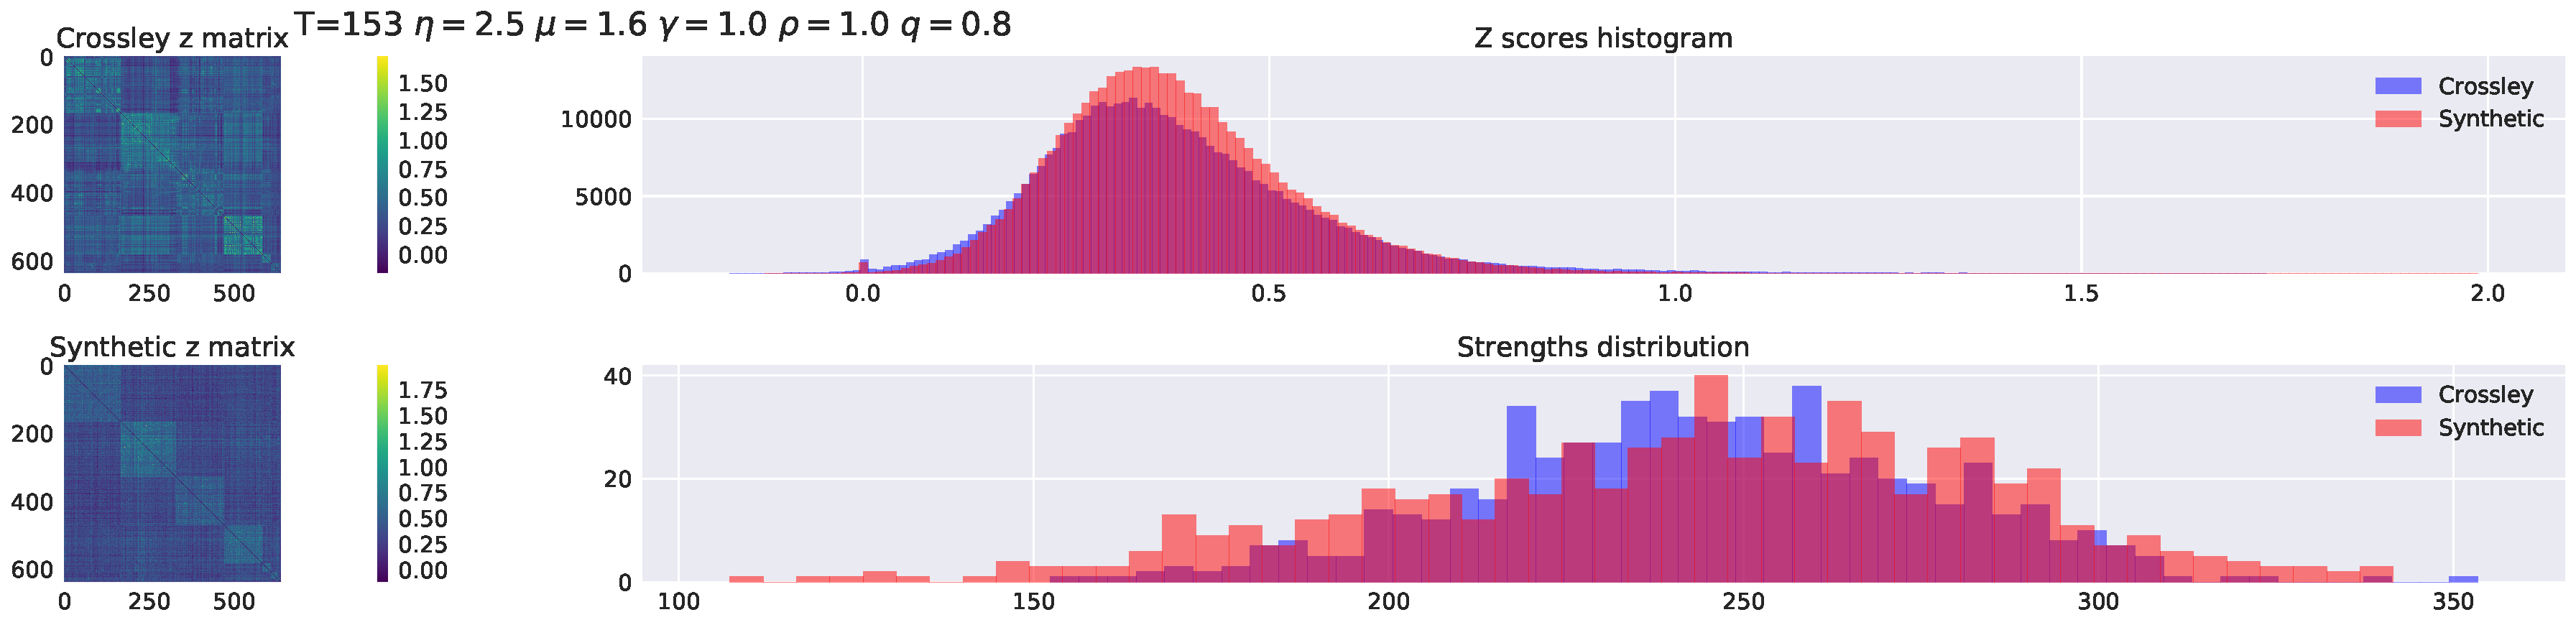
\includegraphics[width=1.0\textwidth]{../crossley_vs_synthetic.pdf}
\caption{Comparison between the crossley z matrix and the synthetic one, with $T=200$ time points, local noise $\eta=2.5$, global noise $\mu=1.5$, soft-threshold coefficient $\gamma=1$ and multiplicative factor $q=0.8$.}
\label{fig:benchmark_network}
\end{figure}

These parameters make the factor model simple enough to study in the settings of the spectral entropies method. In Figure~\ref{fig:benchmark_network} a realization of the model is shown that reflects with good confidence the Crossley network.

\section{Spectral entropies as function of the global noise}
The effect of the global noise parameter is to introduce correlation between all the time-series, resulting in a shift in the global z-score and effects on the spectral entropy. 
Here we try to hypothesize the following phenomenon. As an effect of global correlation increase, with increasing edge weights, the diffusion properties of the network are changing. In particular, with higher ``flux'' on the edges, the diffusion is faster, hence higher entropy is reached at smaller $\beta$.

\begin{figure}
%\includegraphics[width=1.0\textwidth]{../spectral_entropy_synthetic_global_noise.pdf}
\caption{Increase in the global noise. The increase of the intermodule links weights, modifies the spectral entropy, inducing lower entropy at all scales.}
\label{fig:benchmark_network}
\end{figure}


\end{document}
